% VarDial 2027 submission (ACL style, anonymous review). Build: bash build.sh (in this folder)
% Numbers, tables and the figure are those of the full paper (../generated, ../figures), produced by
% ../scripts/make_assets.py from the results files; nothing is typed by hand.
\documentclass[11pt]{article}
\usepackage[review]{acl}
\usepackage{times}
\usepackage{latexsym}
\usepackage[T1]{fontenc}
\usepackage[utf8]{inputenc}
\usepackage{microtype}
\IfFileExists{inconsolata.sty}{\usepackage{inconsolata}}{}
\usepackage{graphicx}
\usepackage{booktabs}
\usepackage{adjustbox}
\usepackage{amsmath}
\usepackage{xspace}
\usepackage{enumitem}
\usepackage[capitalise,noabbrev]{cleveref}
\setlist{itemsep=1pt, topsep=2pt}
\xspaceaddexceptions{\%}
\graphicspath{{../}}
\makeatletter\newcommand{\rawinput}{\@@input}\makeatother
% generated by scripts/make_assets.py -- do not edit
\newcommand{\R}[1]{\ifcsname R@#1\endcsname\csname R@#1\endcsname\else\textbf{??}\fi}
\expandafter\def\csname R@ab:chunk:retries\endcsname{0}
\expandafter\def\csname R@ab:full:cs:c1\endcsname{94\%}
\expandafter\def\csname R@ab:full:cs:cer_canonical\endcsname{0.074}
\expandafter\def\csname R@ab:full:egy_digits:err\endcsname{0.073}
\expandafter\def\csname R@ab:full:egy_main:c1\endcsname{89\%}
\expandafter\def\csname R@ab:full:egy_main:err\endcsname{0.030}
\expandafter\def\csname R@ab:full:egy_main:sim_ecapa\endcsname{0.769}
\expandafter\def\csname R@ab:full:en:sim_ecapa\endcsname{0.779}
\expandafter\def\csname R@ab:no_loanwords:cs:c1\endcsname{94\%}
\expandafter\def\csname R@ab:no_loanwords:cs:c1:ci\endcsname{[\ensuremath{-}22, +22]}
\expandafter\def\csname R@ab:no_loanwords:cs:c1:diff\endcsname{+0 points}
\expandafter\def\csname R@ab:no_loanwords:cs:cer_canonical\endcsname{0.069}
\expandafter\def\csname R@ab:no_loanwords:cs:cer_canonical:ci\endcsname{[\ensuremath{-}0.023, +0.013]}
\expandafter\def\csname R@ab:no_loanwords:cs:cer_canonical:diff\endcsname{\ensuremath{-}0.005}
\expandafter\def\csname R@ab:no_loanwords:egy_digits:err\endcsname{0.073}
\expandafter\def\csname R@ab:no_loanwords:egy_digits:err:ci\endcsname{[+0.000, +0.000]}
\expandafter\def\csname R@ab:no_loanwords:egy_digits:err:diff\endcsname{+0.000}
\expandafter\def\csname R@ab:no_loanwords:egy_main:c1\endcsname{89\%}
\expandafter\def\csname R@ab:no_loanwords:egy_main:c1:ci\endcsname{[+0, +0]}
\expandafter\def\csname R@ab:no_loanwords:egy_main:c1:diff\endcsname{+0 points}
\expandafter\def\csname R@ab:no_loanwords:egy_main:err\endcsname{0.030}
\expandafter\def\csname R@ab:no_loanwords:egy_main:err:ci\endcsname{[+0.000, +0.000]}
\expandafter\def\csname R@ab:no_loanwords:egy_main:err:diff\endcsname{+0.000}
\expandafter\def\csname R@ab:no_loanwords:egy_main:sim_ecapa\endcsname{0.769}
\expandafter\def\csname R@ab:no_loanwords:egy_main:sim_ecapa:ci\endcsname{[+0.000, +0.000]}
\expandafter\def\csname R@ab:no_loanwords:egy_main:sim_ecapa:diff\endcsname{+0.000}
\expandafter\def\csname R@ab:no_loanwords:en:sim_ecapa\endcsname{0.779}
\expandafter\def\csname R@ab:no_loanwords:en:sim_ecapa:ci\endcsname{[+0.000, +0.000]}
\expandafter\def\csname R@ab:no_loanwords:en:sim_ecapa:diff\endcsname{+0.000}
\expandafter\def\csname R@ab:no_normaliser:cs:c1\endcsname{94\%}
\expandafter\def\csname R@ab:no_normaliser:cs:c1:ci\endcsname{[+0, +0]}
\expandafter\def\csname R@ab:no_normaliser:cs:c1:diff\endcsname{+0 points}
\expandafter\def\csname R@ab:no_normaliser:cs:cer_canonical\endcsname{0.074}
\expandafter\def\csname R@ab:no_normaliser:cs:cer_canonical:ci\endcsname{[+0.000, +0.000]}
\expandafter\def\csname R@ab:no_normaliser:cs:cer_canonical:diff\endcsname{+0.000}
\expandafter\def\csname R@ab:no_normaliser:egy_digits:err\endcsname{0.072}
\expandafter\def\csname R@ab:no_normaliser:egy_digits:err:ci\endcsname{[\ensuremath{-}0.035, +0.041]}
\expandafter\def\csname R@ab:no_normaliser:egy_digits:err:diff\endcsname{\ensuremath{-}0.000}
\expandafter\def\csname R@ab:no_normaliser:egy_main:c1\endcsname{89\%}
\expandafter\def\csname R@ab:no_normaliser:egy_main:c1:ci\endcsname{[+0, +0]}
\expandafter\def\csname R@ab:no_normaliser:egy_main:c1:diff\endcsname{+0 points}
\expandafter\def\csname R@ab:no_normaliser:egy_main:err\endcsname{0.030}
\expandafter\def\csname R@ab:no_normaliser:egy_main:err:ci\endcsname{[+0.000, +0.000]}
\expandafter\def\csname R@ab:no_normaliser:egy_main:err:diff\endcsname{+0.000}
\expandafter\def\csname R@ab:no_normaliser:egy_main:sim_ecapa\endcsname{0.769}
\expandafter\def\csname R@ab:no_normaliser:egy_main:sim_ecapa:ci\endcsname{[+0.000, +0.000]}
\expandafter\def\csname R@ab:no_normaliser:egy_main:sim_ecapa:diff\endcsname{+0.000}
\expandafter\def\csname R@ab:no_normaliser:en:sim_ecapa\endcsname{0.780}
\expandafter\def\csname R@ab:no_normaliser:en:sim_ecapa:ci\endcsname{[\ensuremath{-}0.002, +0.004]}
\expandafter\def\csname R@ab:no_normaliser:en:sim_ecapa:diff\endcsname{+0.001}
\expandafter\def\csname R@ab:no_transcript:cs:c1\endcsname{61\%}
\expandafter\def\csname R@ab:no_transcript:cs:c1:ci\endcsname{[\ensuremath{-}67, \ensuremath{-}5]}
\expandafter\def\csname R@ab:no_transcript:cs:c1:diff\endcsname{\ensuremath{-}33 points}
\expandafter\def\csname R@ab:no_transcript:cs:cer_canonical\endcsname{0.121}
\expandafter\def\csname R@ab:no_transcript:cs:cer_canonical:ci\endcsname{[+0.004, +0.108]}
\expandafter\def\csname R@ab:no_transcript:cs:cer_canonical:diff\endcsname{+0.048}
\expandafter\def\csname R@ab:no_transcript:egy_digits:err\endcsname{0.082}
\expandafter\def\csname R@ab:no_transcript:egy_digits:err:ci\endcsname{[\ensuremath{-}0.031, +0.059]}
\expandafter\def\csname R@ab:no_transcript:egy_digits:err:diff\endcsname{+0.010}
\expandafter\def\csname R@ab:no_transcript:egy_main:c1\endcsname{86\%}
\expandafter\def\csname R@ab:no_transcript:egy_main:c1:ci\endcsname{[\ensuremath{-}19, +11]}
\expandafter\def\csname R@ab:no_transcript:egy_main:c1:diff\endcsname{\ensuremath{-}3 points}
\expandafter\def\csname R@ab:no_transcript:egy_main:err\endcsname{0.051}
\expandafter\def\csname R@ab:no_transcript:egy_main:err:ci\endcsname{[\ensuremath{-}0.014, +0.061]}
\expandafter\def\csname R@ab:no_transcript:egy_main:err:diff\endcsname{+0.022}
\expandafter\def\csname R@ab:no_transcript:egy_main:sim_ecapa\endcsname{0.732}
\expandafter\def\csname R@ab:no_transcript:egy_main:sim_ecapa:ci\endcsname{[\ensuremath{-}0.061, \ensuremath{-}0.015]}
\expandafter\def\csname R@ab:no_transcript:egy_main:sim_ecapa:diff\endcsname{\ensuremath{-}0.038}
\expandafter\def\csname R@ab:no_transcript:en:sim_ecapa\endcsname{0.716}
\expandafter\def\csname R@ab:no_transcript:en:sim_ecapa:ci\endcsname{[\ensuremath{-}0.101, \ensuremath{-}0.038]}
\expandafter\def\csname R@ab:no_transcript:en:sim_ecapa:diff\endcsname{\ensuremath{-}0.064}
\expandafter\def\csname R@ab:raw_reference:cs:c1\endcsname{94\%}
\expandafter\def\csname R@ab:raw_reference:cs:c1:ci\endcsname{[\ensuremath{-}22, +22]}
\expandafter\def\csname R@ab:raw_reference:cs:c1:diff\endcsname{+0 points}
\expandafter\def\csname R@ab:raw_reference:cs:cer_canonical\endcsname{0.083}
\expandafter\def\csname R@ab:raw_reference:cs:cer_canonical:ci\endcsname{[\ensuremath{-}0.001, +0.024]}
\expandafter\def\csname R@ab:raw_reference:cs:cer_canonical:diff\endcsname{+0.009}
\expandafter\def\csname R@ab:raw_reference:egy_digits:err\endcsname{0.060}
\expandafter\def\csname R@ab:raw_reference:egy_digits:err:ci\endcsname{[\ensuremath{-}0.041, +0.019]}
\expandafter\def\csname R@ab:raw_reference:egy_digits:err:diff\endcsname{\ensuremath{-}0.012}
\expandafter\def\csname R@ab:raw_reference:egy_main:c1\endcsname{90\%}
\expandafter\def\csname R@ab:raw_reference:egy_main:c1:ci\endcsname{[\ensuremath{-}14, +17]}
\expandafter\def\csname R@ab:raw_reference:egy_main:c1:diff\endcsname{+1 points}
\expandafter\def\csname R@ab:raw_reference:egy_main:err\endcsname{0.023}
\expandafter\def\csname R@ab:raw_reference:egy_main:err:ci\endcsname{[\ensuremath{-}0.033, +0.013]}
\expandafter\def\csname R@ab:raw_reference:egy_main:err:diff\endcsname{\ensuremath{-}0.007}
\expandafter\def\csname R@ab:raw_reference:egy_main:sim_ecapa\endcsname{0.768}
\expandafter\def\csname R@ab:raw_reference:egy_main:sim_ecapa:ci\endcsname{[\ensuremath{-}0.018, +0.013]}
\expandafter\def\csname R@ab:raw_reference:egy_main:sim_ecapa:diff\endcsname{\ensuremath{-}0.001}
\expandafter\def\csname R@ab:raw_reference:en:sim_ecapa\endcsname{0.766}
\expandafter\def\csname R@ab:raw_reference:en:sim_ecapa:ci\endcsname{[\ensuremath{-}0.029, +0.001]}
\expandafter\def\csname R@ab:raw_reference:en:sim_ecapa:diff\endcsname{\ensuremath{-}0.013}
\expandafter\def\csname R@ab:raw_voxcpm2:cs:c1\endcsname{72\%}
\expandafter\def\csname R@ab:raw_voxcpm2:cs:c1:ci\endcsname{[\ensuremath{-}56, +0]}
\expandafter\def\csname R@ab:raw_voxcpm2:cs:c1:diff\endcsname{\ensuremath{-}22 points}
\expandafter\def\csname R@ab:raw_voxcpm2:cs:cer_canonical\endcsname{0.084}
\expandafter\def\csname R@ab:raw_voxcpm2:cs:cer_canonical:ci\endcsname{[\ensuremath{-}0.034, +0.058]}
\expandafter\def\csname R@ab:raw_voxcpm2:cs:cer_canonical:diff\endcsname{+0.011}
\expandafter\def\csname R@ab:raw_voxcpm2:egy_digits:err\endcsname{0.122}
\expandafter\def\csname R@ab:raw_voxcpm2:egy_digits:err:ci\endcsname{[\ensuremath{-}0.012, +0.138]}
\expandafter\def\csname R@ab:raw_voxcpm2:egy_digits:err:diff\endcsname{+0.050}
\expandafter\def\csname R@ab:raw_voxcpm2:egy_main:c1\endcsname{82\%}
\expandafter\def\csname R@ab:raw_voxcpm2:egy_main:c1:ci\endcsname{[\ensuremath{-}27, +12]}
\expandafter\def\csname R@ab:raw_voxcpm2:egy_main:c1:diff\endcsname{\ensuremath{-}7 points}
\expandafter\def\csname R@ab:raw_voxcpm2:egy_main:err\endcsname{0.069}
\expandafter\def\csname R@ab:raw_voxcpm2:egy_main:err:ci\endcsname{[+0.003, +0.095]}
\expandafter\def\csname R@ab:raw_voxcpm2:egy_main:err:diff\endcsname{+0.039}
\expandafter\def\csname R@ab:raw_voxcpm2:egy_main:sim_ecapa\endcsname{0.713}
\expandafter\def\csname R@ab:raw_voxcpm2:egy_main:sim_ecapa:ci\endcsname{[\ensuremath{-}0.081, \ensuremath{-}0.033]}
\expandafter\def\csname R@ab:raw_voxcpm2:egy_main:sim_ecapa:diff\endcsname{\ensuremath{-}0.057}
\expandafter\def\csname R@ab:raw_voxcpm2:en:sim_ecapa\endcsname{0.655}
\expandafter\def\csname R@ab:raw_voxcpm2:en:sim_ecapa:ci\endcsname{[\ensuremath{-}0.245, \ensuremath{-}0.050]}
\expandafter\def\csname R@ab:raw_voxcpm2:en:sim_ecapa:diff\endcsname{\ensuremath{-}0.124}
\expandafter\def\csname R@ab:share:notrans:cer\endcsname{55\%}
\expandafter\def\csname R@ab:share:notrans:ecapa\endcsname{67\%}
\expandafter\def\csname R@asr:large:cer\endcsname{0.071}
\expandafter\def\csname R@asr:turbo:cer\endcsname{0.070}
\expandafter\def\csname R@bench:arz:audio\endcsname{9.4}
\expandafter\def\csname R@bench:arz:time\endcsname{6.3}
\expandafter\def\csname R@bench:arz:words\endcsname{23}
\expandafter\def\csname R@bench:arzlong:audio\endcsname{41.1}
\expandafter\def\csname R@bench:arzlong:time\endcsname{27.5}
\expandafter\def\csname R@bench:arzlong:words\endcsname{118}
\expandafter\def\csname R@bench:load\endcsname{33}
\expandafter\def\csname R@bench:voice\endcsname{0.29}
\expandafter\def\csname R@bench:vram\endcsname{8.11}
\expandafter\def\csname R@bk:cb-v2:c1pct\endcsname{17\%}
\expandafter\def\csname R@bk:cb-v2:c2pct\endcsname{40\%}
\expandafter\def\csname R@bk:cb-v2:cer\endcsname{0.056}
\expandafter\def\csname R@bk:cb-v2:ecapa\endcsname{0.739}
\expandafter\def\csname R@bk:cb-v2:fail\endcsname{3.1\%}
\expandafter\def\csname R@bk:cb-v2:kappa\endcsname{0.27}
\expandafter\def\csname R@bk:cb-v2:mos\endcsname{3.60}
\expandafter\def\csname R@bk:cb-v3-pypi:c1pct\endcsname{25\%}
\expandafter\def\csname R@bk:cb-v3-pypi:c2pct\endcsname{45\%}
\expandafter\def\csname R@bk:cb-v3-pypi:cer\endcsname{0.230}
\expandafter\def\csname R@bk:cb-v3-pypi:ecapa\endcsname{0.682}
\expandafter\def\csname R@bk:cb-v3-pypi:fail\endcsname{23.5\%}
\expandafter\def\csname R@bk:cb-v3-pypi:kappa\endcsname{0.32}
\expandafter\def\csname R@bk:cb-v3-pypi:mos\endcsname{3.44}
\expandafter\def\csname R@bk:cb-v3:c1pct\endcsname{21\%}
\expandafter\def\csname R@bk:cb-v3:c2pct\endcsname{51\%}
\expandafter\def\csname R@bk:cb-v3:cer\endcsname{0.035}
\expandafter\def\csname R@bk:cb-v3:ecapa\endcsname{0.706}
\expandafter\def\csname R@bk:cb-v3:fail\endcsname{1.8\%}
\expandafter\def\csname R@bk:cb-v3:kappa\endcsname{0.20}
\expandafter\def\csname R@bk:cb-v3:mos\endcsname{3.66}
\expandafter\def\csname R@bk:lahgtna:c1pct\endcsname{20\%}
\expandafter\def\csname R@bk:lahgtna:c2pct\endcsname{45\%}
\expandafter\def\csname R@bk:lahgtna:cer\endcsname{0.442}
\expandafter\def\csname R@bk:lahgtna:ecapa\endcsname{0.742}
\expandafter\def\csname R@bk:lahgtna:fail\endcsname{6.9\%}
\expandafter\def\csname R@bk:lahgtna:kappa\endcsname{0.33}
\expandafter\def\csname R@bk:lahgtna:mos\endcsname{3.51}
\expandafter\def\csname R@bk:namaa:c1pct\endcsname{93\%}
\expandafter\def\csname R@bk:namaa:c2pct\endcsname{97\%}
\expandafter\def\csname R@bk:namaa:cer\endcsname{0.082}
\expandafter\def\csname R@bk:namaa:ecapa\endcsname{0.721}
\expandafter\def\csname R@bk:namaa:fail\endcsname{0.6\%}
\expandafter\def\csname R@bk:namaa:kappa\endcsname{0.16}
\expandafter\def\csname R@bk:namaa:mos\endcsname{3.47}
\expandafter\def\csname R@bk:omnivoice:c1pct\endcsname{82\%}
\expandafter\def\csname R@bk:omnivoice:c2pct\endcsname{90\%}
\expandafter\def\csname R@bk:omnivoice:cer\endcsname{0.083}
\expandafter\def\csname R@bk:omnivoice:ecapa\endcsname{0.773}
\expandafter\def\csname R@bk:omnivoice:fail\endcsname{0.0\%}
\expandafter\def\csname R@bk:omnivoice:kappa\endcsname{0.10}
\expandafter\def\csname R@bk:omnivoice:mos\endcsname{3.65}
\expandafter\def\csname R@bk:voicetut:c1pct\endcsname{90\%}
\expandafter\def\csname R@bk:voicetut:c2pct\endcsname{97\%}
\expandafter\def\csname R@bk:voicetut:cer\endcsname{0.079}
\expandafter\def\csname R@bk:voicetut:ecapa\endcsname{0.713}
\expandafter\def\csname R@bk:voicetut:fail\endcsname{0.9\%}
\expandafter\def\csname R@bk:voicetut:kappa\endcsname{0.27}
\expandafter\def\csname R@bk:voicetut:mos\endcsname{3.65}
\expandafter\def\csname R@bk:voxcpm2-prompt:c1pct\endcsname{91\%}
\expandafter\def\csname R@bk:voxcpm2-prompt:c2pct\endcsname{71\%}
\expandafter\def\csname R@bk:voxcpm2-prompt:cer\endcsname{0.080}
\expandafter\def\csname R@bk:voxcpm2-prompt:ecapa\endcsname{0.769}
\expandafter\def\csname R@bk:voxcpm2-prompt:fail\endcsname{0.0\%}
\expandafter\def\csname R@bk:voxcpm2-prompt:kappa\endcsname{0.02}
\expandafter\def\csname R@bk:voxcpm2-prompt:mos\endcsname{3.46}
\expandafter\def\csname R@bk:voxcpm2:c1pct\endcsname{82\%}
\expandafter\def\csname R@bk:voxcpm2:c2pct\endcsname{74\%}
\expandafter\def\csname R@bk:voxcpm2:cer\endcsname{0.065}
\expandafter\def\csname R@bk:voxcpm2:cpurtf\endcsname{31}
\expandafter\def\csname R@bk:voxcpm2:ecapa\endcsname{0.714}
\expandafter\def\csname R@bk:voxcpm2:fail\endcsname{0.9\%}
\expandafter\def\csname R@bk:voxcpm2:kappa\endcsname{0.09}
\expandafter\def\csname R@bk:voxcpm2:mos\endcsname{3.35}
\expandafter\def\csname R@cal:fleurs:c1pct\endcsname{34\%}
\expandafter\def\csname R@cal:fleurs:c2pct\endcsname{42\%}
\expandafter\def\csname R@cal:fleurs:cer\endcsname{0.014}
\expandafter\def\csname R@cal:lahgtna:c1pct\endcsname{90\%}
\expandafter\def\csname R@cal:lahgtna:c2pct\endcsname{98\%}
\expandafter\def\csname R@cal:lahgtna:cer\endcsname{0.071}
\expandafter\def\csname R@cal:niletts:c1pct\endcsname{98\%}
\expandafter\def\csname R@cal:niletts:c2pct\endcsname{100\%}
\expandafter\def\csname R@cal:niletts:cer\endcsname{0.019}
\expandafter\def\csname R@cal:spk:ceiling\endcsname{0.870}
\expandafter\def\csname R@cal:spk:floor\endcsname{0.184}
\expandafter\def\csname R@chunk:maxchars\endcsname{1,000}
\expandafter\def\csname R@cs:arabic:c1pct\endcsname{79\%}
\expandafter\def\csname R@cs:arabic:cer\endcsname{0.093}
\expandafter\def\csname R@cs:keep:c1pct\endcsname{71\%}
\expandafter\def\csname R@cs:keep:cer\endcsname{0.092}
\expandafter\def\csname R@g1:bar\endcsname{54\%}
\expandafter\def\csname R@g3:arz:cerbar\endcsname{0.171}
\expandafter\def\csname R@g3:arz:simbar\endcsname{0.696}
\expandafter\def\csname R@g3:en:simbar\endcsname{0.699}
\expandafter\def\csname R@g3:fr:simbar\endcsname{0.720}
\expandafter\def\csname R@ho:ba:c1pct\endcsname{89\%}
\expandafter\def\csname R@ho:ba:cer\endcsname{0.030}
\expandafter\def\csname R@ho:ba:cs:c1pct\endcsname{94\%}
\expandafter\def\csname R@ho:ba:cs:cer\endcsname{0.284}
\expandafter\def\csname R@ho:ba:diac:c1pct\endcsname{60\%}
\expandafter\def\csname R@ho:ba:diac:cer\endcsname{0.040}
\expandafter\def\csname R@ho:ba:ecapa\endcsname{0.769}
\expandafter\def\csname R@ho:ba:en:ecapa\endcsname{0.779}
\expandafter\def\csname R@ho:ba:en:fail\endcsname{0 of 42}
\expandafter\def\csname R@ho:ba:en:wer\endcsname{0.003}
\expandafter\def\csname R@ho:ba:fr:ecapa\endcsname{0.792}
\expandafter\def\csname R@ho:ba:fr:fail\endcsname{0 of 60}
\expandafter\def\csname R@ho:ba:fr:wer\endcsname{0.030}
\expandafter\def\csname R@ho:ba:mos\endcsname{3.53}
\expandafter\def\csname R@ho:voxcpm2:c1pct\endcsname{82\%}
\expandafter\def\csname R@ho:voxcpm2:cer\endcsname{0.069}
\expandafter\def\csname R@ho:voxcpm2:cs:c1pct\endcsname{72\%}
\expandafter\def\csname R@ho:voxcpm2:cs:cer\endcsname{0.274}
\expandafter\def\csname R@ho:voxcpm2:diac:c1pct\endcsname{40\%}
\expandafter\def\csname R@ho:voxcpm2:diac:cer\endcsname{0.045}
\expandafter\def\csname R@ho:voxcpm2:ecapa\endcsname{0.713}
\expandafter\def\csname R@ho:voxcpm2:en:ecapa\endcsname{0.655}
\expandafter\def\csname R@ho:voxcpm2:en:fail\endcsname{2 of 42}
\expandafter\def\csname R@ho:voxcpm2:en:wer\endcsname{0.000}
\expandafter\def\csname R@ho:voxcpm2:fr:ecapa\endcsname{0.759}
\expandafter\def\csname R@ho:voxcpm2:fr:fail\endcsname{0 of 60}
\expandafter\def\csname R@ho:voxcpm2:fr:wer\endcsname{0.030}
\expandafter\def\csname R@ho:voxcpm2:mos\endcsname{3.35}
\expandafter\def\csname R@ho:voxcpm2p:c1pct\endcsname{90\%}
\expandafter\def\csname R@ho:voxcpm2p:cer\endcsname{0.079}
\expandafter\def\csname R@ho:voxcpm2p:ecapa\endcsname{0.771}
\expandafter\def\csname R@ho:voxcpm2p:mos\endcsname{3.44}
\expandafter\def\csname R@hodig:ba:c1pct\endcsname{83\%}
\expandafter\def\csname R@hodig:ba:cer\endcsname{0.073}
\expandafter\def\csname R@hodig:ba:ecapa\endcsname{0.777}
\expandafter\def\csname R@hodig:ba:mos\endcsname{3.56}
\expandafter\def\csname R@hodig:voxcpm2:c1pct\endcsname{67\%}
\expandafter\def\csname R@hodig:voxcpm2:cer\endcsname{0.122}
\expandafter\def\csname R@hodig:voxcpm2:ecapa\endcsname{0.730}
\expandafter\def\csname R@hodig:voxcpm2:mos\endcsname{3.31}
\expandafter\def\csname R@hodig:voxcpm2p:c1pct\endcsname{89\%}
\expandafter\def\csname R@hodig:voxcpm2p:cer\endcsname{0.152}
\expandafter\def\csname R@hodig:voxcpm2p:ecapa\endcsname{0.780}
\expandafter\def\csname R@hodig:voxcpm2p:mos\endcsname{3.45}
\expandafter\def\csname R@kappa:gen\endcsname{0.46}
\expandafter\def\csname R@kappa:real\endcsname{0.64}
\expandafter\def\csname R@lab:cb-v2:Egyptian\endcsname{17\%}
\expandafter\def\csname R@lab:cb-v2:Gulf\endcsname{18\%}
\expandafter\def\csname R@lab:cb-v2:Levantine\endcsname{34\%}
\expandafter\def\csname R@lab:cb-v2:MSA\endcsname{25\%}
\expandafter\def\csname R@lab:cb-v2:Maghrebi\endcsname{6\%}
\expandafter\def\csname R@lab:cb-v3-pypi:Egyptian\endcsname{25\%}
\expandafter\def\csname R@lab:cb-v3-pypi:Gulf\endcsname{24\%}
\expandafter\def\csname R@lab:cb-v3-pypi:Levantine\endcsname{32\%}
\expandafter\def\csname R@lab:cb-v3-pypi:MSA\endcsname{9\%}
\expandafter\def\csname R@lab:cb-v3-pypi:Maghrebi\endcsname{9\%}
\expandafter\def\csname R@lab:cb-v3:Egyptian\endcsname{21\%}
\expandafter\def\csname R@lab:cb-v3:Gulf\endcsname{21\%}
\expandafter\def\csname R@lab:cb-v3:Levantine\endcsname{34\%}
\expandafter\def\csname R@lab:cb-v3:MSA\endcsname{17\%}
\expandafter\def\csname R@lab:cb-v3:Maghrebi\endcsname{7\%}
\expandafter\def\csname R@lab:chat:lev\endcsname{44\%}
\expandafter\def\csname R@lab:lahgtna:Egyptian\endcsname{20\%}
\expandafter\def\csname R@lab:lahgtna:Gulf\endcsname{11\%}
\expandafter\def\csname R@lab:lahgtna:Levantine\endcsname{62\%}
\expandafter\def\csname R@lab:lahgtna:MSA\endcsname{1\%}
\expandafter\def\csname R@lab:lahgtna:Maghrebi\endcsname{5\%}
\expandafter\def\csname R@lab:namaa:Egyptian\endcsname{93\%}
\expandafter\def\csname R@lab:namaa:Gulf\endcsname{4\%}
\expandafter\def\csname R@lab:namaa:Levantine\endcsname{2\%}
\expandafter\def\csname R@lab:namaa:MSA\endcsname{0\%}
\expandafter\def\csname R@lab:namaa:Maghrebi\endcsname{1\%}
\expandafter\def\csname R@lab:omnivoice:Egyptian\endcsname{82\%}
\expandafter\def\csname R@lab:omnivoice:Gulf\endcsname{6\%}
\expandafter\def\csname R@lab:omnivoice:Levantine\endcsname{9\%}
\expandafter\def\csname R@lab:omnivoice:MSA\endcsname{2\%}
\expandafter\def\csname R@lab:omnivoice:Maghrebi\endcsname{0\%}
\expandafter\def\csname R@lab:voicetut:Egyptian\endcsname{90\%}
\expandafter\def\csname R@lab:voicetut:Gulf\endcsname{2\%}
\expandafter\def\csname R@lab:voicetut:Levantine\endcsname{5\%}
\expandafter\def\csname R@lab:voicetut:MSA\endcsname{0\%}
\expandafter\def\csname R@lab:voicetut:Maghrebi\endcsname{3\%}
\expandafter\def\csname R@lab:voxcpm2-prompt:Egyptian\endcsname{91\%}
\expandafter\def\csname R@lab:voxcpm2-prompt:Gulf\endcsname{5\%}
\expandafter\def\csname R@lab:voxcpm2-prompt:Levantine\endcsname{4\%}
\expandafter\def\csname R@lab:voxcpm2-prompt:MSA\endcsname{0\%}
\expandafter\def\csname R@lab:voxcpm2-prompt:Maghrebi\endcsname{0\%}
\expandafter\def\csname R@lab:voxcpm2:Egyptian\endcsname{82\%}
\expandafter\def\csname R@lab:voxcpm2:Gulf\endcsname{7\%}
\expandafter\def\csname R@lab:voxcpm2:Levantine\endcsname{8\%}
\expandafter\def\csname R@lab:voxcpm2:MSA\endcsname{1\%}
\expandafter\def\csname R@lab:voxcpm2:Maghrebi\endcsname{1\%}
\expandafter\def\csname R@long1:ba:arz:err\endcsname{0.040}
\expandafter\def\csname R@long1:ba:arz:fail\endcsname{0 of 2}
\expandafter\def\csname R@long1:ba:en:err\endcsname{0.000}
\expandafter\def\csname R@long1:ba:en:fail\endcsname{0 of 2}
\expandafter\def\csname R@long1:ba:fr:err\endcsname{0.010}
\expandafter\def\csname R@long1:ba:fr:fail\endcsname{0 of 2}
\expandafter\def\csname R@long1:voxcpm2:arz:err\endcsname{0.033}
\expandafter\def\csname R@long1:voxcpm2:arz:fail\endcsname{0 of 2}
\expandafter\def\csname R@long1:voxcpm2:en:err\endcsname{0.000}
\expandafter\def\csname R@long1:voxcpm2:en:fail\endcsname{0 of 2}
\expandafter\def\csname R@long1:voxcpm2:fr:err\endcsname{0.010}
\expandafter\def\csname R@long1:voxcpm2:fr:fail\endcsname{0 of 2}
\expandafter\def\csname R@lt:cb-v2:egy\endcsname{0 of 6}
\expandafter\def\csname R@lt:cb-v2:mid\endcsname{0 of 6}
\expandafter\def\csname R@lt:cb-v2:not\endcsname{6 of 6}
\expandafter\def\csname R@lt:cb-v2:words\endcsname{2 of 6}
\expandafter\def\csname R@lt:cb-v3:egy\endcsname{0 of 6}
\expandafter\def\csname R@lt:cb-v3:mid\endcsname{0 of 6}
\expandafter\def\csname R@lt:cb-v3:not\endcsname{6 of 6}
\expandafter\def\csname R@lt:cb-v3:words\endcsname{4 of 6}
\expandafter\def\csname R@lt:lahgtna:egy\endcsname{2 of 6}
\expandafter\def\csname R@lt:lahgtna:mid\endcsname{2 of 6}
\expandafter\def\csname R@lt:lahgtna:not\endcsname{2 of 6}
\expandafter\def\csname R@lt:lahgtna:words\endcsname{4 of 6}
\expandafter\def\csname R@lt:n\endcsname{6}
\expandafter\def\csname R@lt:namaa:egy\endcsname{1 of 6}
\expandafter\def\csname R@lt:namaa:mid\endcsname{3 of 6}
\expandafter\def\csname R@lt:namaa:not\endcsname{2 of 6}
\expandafter\def\csname R@lt:namaa:words\endcsname{4 of 6}
\expandafter\def\csname R@lt:omnivoice:egy\endcsname{2 of 6}
\expandafter\def\csname R@lt:omnivoice:mid\endcsname{3 of 6}
\expandafter\def\csname R@lt:omnivoice:not\endcsname{1 of 6}
\expandafter\def\csname R@lt:omnivoice:words\endcsname{3 of 6}
\expandafter\def\csname R@lt:voicetut:egy\endcsname{3 of 6}
\expandafter\def\csname R@lt:voicetut:mid\endcsname{3 of 6}
\expandafter\def\csname R@lt:voicetut:not\endcsname{0 of 6}
\expandafter\def\csname R@lt:voicetut:words\endcsname{5 of 6}
\expandafter\def\csname R@lt:voxcpm2-prompt:egy\endcsname{1 of 6}
\expandafter\def\csname R@lt:voxcpm2-prompt:mid\endcsname{5 of 6}
\expandafter\def\csname R@lt:voxcpm2-prompt:not\endcsname{0 of 6}
\expandafter\def\csname R@lt:voxcpm2-prompt:words\endcsname{5 of 6}
\expandafter\def\csname R@lt:voxcpm2:egy\endcsname{3 of 6}
\expandafter\def\csname R@lt:voxcpm2:mid\endcsname{3 of 6}
\expandafter\def\csname R@lt:voxcpm2:not\endcsname{0 of 6}
\expandafter\def\csname R@lt:voxcpm2:words\endcsname{3 of 6}
\expandafter\def\csname R@pt:ba_minus_cb-v3:egy_digits:c1:ci\endcsname{[+21, +100]}
\expandafter\def\csname R@pt:ba_minus_cb-v3:egy_digits:c1:diff\endcsname{+72 points}
\expandafter\def\csname R@pt:ba_minus_cb-v3:egy_digits:c1:p\endcsname{p=0.016}
\expandafter\def\csname R@pt:ba_minus_cb-v3:egy_digits:c2:ci\endcsname{[\ensuremath{-}6, +77]}
\expandafter\def\csname R@pt:ba_minus_cb-v3:egy_digits:c2:diff\endcsname{+39 points}
\expandafter\def\csname R@pt:ba_minus_cb-v3:egy_digits:c2:p\endcsname{p=0.110}
\expandafter\def\csname R@pt:ba_minus_cb-v3:egy_digits:cer_best:ci\endcsname{[\ensuremath{-}0.113, +0.004]}
\expandafter\def\csname R@pt:ba_minus_cb-v3:egy_digits:cer_best:diff\endcsname{\ensuremath{-}0.055}
\expandafter\def\csname R@pt:ba_minus_cb-v3:egy_digits:cer_best:p\endcsname{p=0.072}
\expandafter\def\csname R@pt:ba_minus_cb-v3:egy_digits:failed:ci\endcsname{[0, 0]}
\expandafter\def\csname R@pt:ba_minus_cb-v3:egy_digits:failed:diff\endcsname{0 points}
\expandafter\def\csname R@pt:ba_minus_cb-v3:egy_digits:failed:p\endcsname{p=1.000}
\expandafter\def\csname R@pt:ba_minus_cb-v3:egy_digits:mos_p808:ci\endcsname{[\ensuremath{-}0.19, +0.08]}
\expandafter\def\csname R@pt:ba_minus_cb-v3:egy_digits:mos_p808:diff\endcsname{\ensuremath{-}0.05}
\expandafter\def\csname R@pt:ba_minus_cb-v3:egy_digits:mos_p808:p\endcsname{p=0.446}
\expandafter\def\csname R@pt:ba_minus_cb-v3:egy_digits:sim_ecapa:ci\endcsname{[\ensuremath{-}0.000, +0.135]}
\expandafter\def\csname R@pt:ba_minus_cb-v3:egy_digits:sim_ecapa:diff\endcsname{+0.066}
\expandafter\def\csname R@pt:ba_minus_cb-v3:egy_digits:sim_ecapa:p\endcsname{p=0.050}
\expandafter\def\csname R@pt:ba_minus_cb-v3:egy_digits:sim_wavlm:ci\endcsname{[\ensuremath{-}0.013, +0.016]}
\expandafter\def\csname R@pt:ba_minus_cb-v3:egy_digits:sim_wavlm:diff\endcsname{+0.001}
\expandafter\def\csname R@pt:ba_minus_cb-v3:egy_digits:sim_wavlm:p\endcsname{p=0.879}
\expandafter\def\csname R@pt:ba_minus_cb-v3:egy_main:c1:ci\endcsname{[+45, +86]}
\expandafter\def\csname R@pt:ba_minus_cb-v3:egy_main:c1:diff\endcsname{+67 points}
\expandafter\def\csname R@pt:ba_minus_cb-v3:egy_main:c1:p\endcsname{p<0.001}
\expandafter\def\csname R@pt:ba_minus_cb-v3:egy_main:c2:ci\endcsname{[+10, +49]}
\expandafter\def\csname R@pt:ba_minus_cb-v3:egy_main:c2:diff\endcsname{+29 points}
\expandafter\def\csname R@pt:ba_minus_cb-v3:egy_main:c2:p\endcsname{p=0.004}
\expandafter\def\csname R@pt:ba_minus_cb-v3:egy_main:cer_best:ci\endcsname{[\ensuremath{-}0.035, +0.024]}
\expandafter\def\csname R@pt:ba_minus_cb-v3:egy_main:cer_best:diff\endcsname{\ensuremath{-}0.003}
\expandafter\def\csname R@pt:ba_minus_cb-v3:egy_main:cer_best:p\endcsname{p=0.844}
\expandafter\def\csname R@pt:ba_minus_cb-v3:egy_main:failed:ci\endcsname{[0, 0]}
\expandafter\def\csname R@pt:ba_minus_cb-v3:egy_main:failed:diff\endcsname{0 points}
\expandafter\def\csname R@pt:ba_minus_cb-v3:egy_main:failed:p\endcsname{p=1.000}
\expandafter\def\csname R@pt:ba_minus_cb-v3:egy_main:mos_p808:ci\endcsname{[\ensuremath{-}0.22, \ensuremath{-}0.01]}
\expandafter\def\csname R@pt:ba_minus_cb-v3:egy_main:mos_p808:diff\endcsname{\ensuremath{-}0.11}
\expandafter\def\csname R@pt:ba_minus_cb-v3:egy_main:mos_p808:p\endcsname{p=0.033}
\expandafter\def\csname R@pt:ba_minus_cb-v3:egy_main:sim_ecapa:ci\endcsname{[+0.039, +0.105]}
\expandafter\def\csname R@pt:ba_minus_cb-v3:egy_main:sim_ecapa:diff\endcsname{+0.070}
\expandafter\def\csname R@pt:ba_minus_cb-v3:egy_main:sim_ecapa:p\endcsname{p<0.001}
\expandafter\def\csname R@pt:ba_minus_cb-v3:egy_main:sim_wavlm:ci\endcsname{[\ensuremath{-}0.008, +0.006]}
\expandafter\def\csname R@pt:ba_minus_cb-v3:egy_main:sim_wavlm:diff\endcsname{\ensuremath{-}0.001}
\expandafter\def\csname R@pt:ba_minus_cb-v3:egy_main:sim_wavlm:p\endcsname{p=0.894}
\expandafter\def\csname R@pt:ba_minus_voxcpm2:egy_digits:c1:ci\endcsname{[\ensuremath{-}25, +50]}
\expandafter\def\csname R@pt:ba_minus_voxcpm2:egy_digits:c1:diff\endcsname{+17 points}
\expandafter\def\csname R@pt:ba_minus_voxcpm2:egy_digits:c1:p\endcsname{p=0.462}
\expandafter\def\csname R@pt:ba_minus_voxcpm2:egy_digits:c2:ci\endcsname{[\ensuremath{-}56, +50]}
\expandafter\def\csname R@pt:ba_minus_voxcpm2:egy_digits:c2:diff\endcsname{0 points}
\expandafter\def\csname R@pt:ba_minus_voxcpm2:egy_digits:c2:p\endcsname{p=1.000}
\expandafter\def\csname R@pt:ba_minus_voxcpm2:egy_digits:cer_best:ci\endcsname{[\ensuremath{-}0.138, +0.012]}
\expandafter\def\csname R@pt:ba_minus_voxcpm2:egy_digits:cer_best:diff\endcsname{\ensuremath{-}0.050}
\expandafter\def\csname R@pt:ba_minus_voxcpm2:egy_digits:cer_best:p\endcsname{p=0.146}
\expandafter\def\csname R@pt:ba_minus_voxcpm2:egy_digits:failed:ci\endcsname{[0, 0]}
\expandafter\def\csname R@pt:ba_minus_voxcpm2:egy_digits:failed:diff\endcsname{0 points}
\expandafter\def\csname R@pt:ba_minus_voxcpm2:egy_digits:failed:p\endcsname{p=1.000}
\expandafter\def\csname R@pt:ba_minus_voxcpm2:egy_digits:mos_p808:ci\endcsname{[+0.03, +0.38]}
\expandafter\def\csname R@pt:ba_minus_voxcpm2:egy_digits:mos_p808:diff\endcsname{+0.25}
\expandafter\def\csname R@pt:ba_minus_voxcpm2:egy_digits:mos_p808:p\endcsname{p=0.035}
\expandafter\def\csname R@pt:ba_minus_voxcpm2:egy_digits:sim_ecapa:ci\endcsname{[+0.011, +0.092]}
\expandafter\def\csname R@pt:ba_minus_voxcpm2:egy_digits:sim_ecapa:diff\endcsname{+0.047}
\expandafter\def\csname R@pt:ba_minus_voxcpm2:egy_digits:sim_ecapa:p\endcsname{p=0.002}
\expandafter\def\csname R@pt:ba_minus_voxcpm2:egy_digits:sim_wavlm:ci\endcsname{[\ensuremath{-}0.004, +0.020]}
\expandafter\def\csname R@pt:ba_minus_voxcpm2:egy_digits:sim_wavlm:diff\endcsname{+0.007}
\expandafter\def\csname R@pt:ba_minus_voxcpm2:egy_digits:sim_wavlm:p\endcsname{p=0.226}
\expandafter\def\csname R@pt:ba_minus_voxcpm2:egy_main:c1:ci\endcsname{[\ensuremath{-}12, +27]}
\expandafter\def\csname R@pt:ba_minus_voxcpm2:egy_main:c1:diff\endcsname{+7 points}
\expandafter\def\csname R@pt:ba_minus_voxcpm2:egy_main:c1:p\endcsname{p=0.490}
\expandafter\def\csname R@pt:ba_minus_voxcpm2:egy_main:c1:pholm\endcsname{p_{\mathrm{Holm}}=0.490}
\expandafter\def\csname R@pt:ba_minus_voxcpm2:egy_main:c2:ci\endcsname{[\ensuremath{-}13, +25]}
\expandafter\def\csname R@pt:ba_minus_voxcpm2:egy_main:c2:diff\endcsname{+7 points}
\expandafter\def\csname R@pt:ba_minus_voxcpm2:egy_main:c2:p\endcsname{p=0.463}
\expandafter\def\csname R@pt:ba_minus_voxcpm2:egy_main:cer_best:ci\endcsname{[\ensuremath{-}0.095, \ensuremath{-}0.003]}
\expandafter\def\csname R@pt:ba_minus_voxcpm2:egy_main:cer_best:diff\endcsname{\ensuremath{-}0.039}
\expandafter\def\csname R@pt:ba_minus_voxcpm2:egy_main:cer_best:p\endcsname{p=0.033}
\expandafter\def\csname R@pt:ba_minus_voxcpm2:egy_main:cer_best:pholm\endcsname{p_{\mathrm{Holm}}=0.098}
\expandafter\def\csname R@pt:ba_minus_voxcpm2:egy_main:failed:ci\endcsname{[0, 0]}
\expandafter\def\csname R@pt:ba_minus_voxcpm2:egy_main:failed:diff\endcsname{0 points}
\expandafter\def\csname R@pt:ba_minus_voxcpm2:egy_main:failed:p\endcsname{p=1.000}
\expandafter\def\csname R@pt:ba_minus_voxcpm2:egy_main:mos_p808:ci\endcsname{[+0.06, +0.29]}
\expandafter\def\csname R@pt:ba_minus_voxcpm2:egy_main:mos_p808:diff\endcsname{+0.18}
\expandafter\def\csname R@pt:ba_minus_voxcpm2:egy_main:mos_p808:p\endcsname{p=0.004}
\expandafter\def\csname R@pt:ba_minus_voxcpm2:egy_main:sim_ecapa:ci\endcsname{[+0.033, +0.081]}
\expandafter\def\csname R@pt:ba_minus_voxcpm2:egy_main:sim_ecapa:diff\endcsname{+0.057}
\expandafter\def\csname R@pt:ba_minus_voxcpm2:egy_main:sim_ecapa:p\endcsname{p<0.001}
\expandafter\def\csname R@pt:ba_minus_voxcpm2:egy_main:sim_ecapa:pholm\endcsname{p_{\mathrm{Holm}}<0.001}
\expandafter\def\csname R@pt:ba_minus_voxcpm2:egy_main:sim_wavlm:ci\endcsname{[\ensuremath{-}0.000, +0.018]}
\expandafter\def\csname R@pt:ba_minus_voxcpm2:egy_main:sim_wavlm:diff\endcsname{+0.008}
\expandafter\def\csname R@pt:ba_minus_voxcpm2:egy_main:sim_wavlm:p\endcsname{p=0.055}
\expandafter\def\csname R@pt:voxcpm2_minus_cb-v3:egy_digits:c1:ci\endcsname{[0, +100]}
\expandafter\def\csname R@pt:voxcpm2_minus_cb-v3:egy_digits:c1:diff\endcsname{+56 points}
\expandafter\def\csname R@pt:voxcpm2_minus_cb-v3:egy_digits:c1:p\endcsname{p=0.063}
\expandafter\def\csname R@pt:voxcpm2_minus_cb-v3:egy_digits:c2:ci\endcsname{[\ensuremath{-}6, +80]}
\expandafter\def\csname R@pt:voxcpm2_minus_cb-v3:egy_digits:c2:diff\endcsname{+39 points}
\expandafter\def\csname R@pt:voxcpm2_minus_cb-v3:egy_digits:c2:p\endcsname{p=0.120}
\expandafter\def\csname R@pt:voxcpm2_minus_cb-v3:egy_digits:cer_best:ci\endcsname{[\ensuremath{-}0.081, +0.093]}
\expandafter\def\csname R@pt:voxcpm2_minus_cb-v3:egy_digits:cer_best:diff\endcsname{\ensuremath{-}0.005}
\expandafter\def\csname R@pt:voxcpm2_minus_cb-v3:egy_digits:cer_best:p\endcsname{p=0.818}
\expandafter\def\csname R@pt:voxcpm2_minus_cb-v3:egy_digits:failed:ci\endcsname{[0, 0]}
\expandafter\def\csname R@pt:voxcpm2_minus_cb-v3:egy_digits:failed:diff\endcsname{0 points}
\expandafter\def\csname R@pt:voxcpm2_minus_cb-v3:egy_digits:failed:p\endcsname{p=1.000}
\expandafter\def\csname R@pt:voxcpm2_minus_cb-v3:egy_digits:mos_p808:ci\endcsname{[\ensuremath{-}0.45, \ensuremath{-}0.13]}
\expandafter\def\csname R@pt:voxcpm2_minus_cb-v3:egy_digits:mos_p808:diff\endcsname{\ensuremath{-}0.30}
\expandafter\def\csname R@pt:voxcpm2_minus_cb-v3:egy_digits:mos_p808:p\endcsname{p<0.001}
\expandafter\def\csname R@pt:voxcpm2_minus_cb-v3:egy_digits:sim_ecapa:ci\endcsname{[\ensuremath{-}0.057, +0.109]}
\expandafter\def\csname R@pt:voxcpm2_minus_cb-v3:egy_digits:sim_ecapa:diff\endcsname{+0.019}
\expandafter\def\csname R@pt:voxcpm2_minus_cb-v3:egy_digits:sim_ecapa:p\endcsname{p=0.665}
\expandafter\def\csname R@pt:voxcpm2_minus_cb-v3:egy_digits:sim_wavlm:ci\endcsname{[\ensuremath{-}0.024, +0.011]}
\expandafter\def\csname R@pt:voxcpm2_minus_cb-v3:egy_digits:sim_wavlm:diff\endcsname{\ensuremath{-}0.006}
\expandafter\def\csname R@pt:voxcpm2_minus_cb-v3:egy_digits:sim_wavlm:p\endcsname{p=0.431}
\expandafter\def\csname R@pt:voxcpm2_minus_cb-v3:egy_main:c1:ci\endcsname{[+31, +86]}
\expandafter\def\csname R@pt:voxcpm2_minus_cb-v3:egy_main:c1:diff\endcsname{+60 points}
\expandafter\def\csname R@pt:voxcpm2_minus_cb-v3:egy_main:c1:p\endcsname{p<0.001}
\expandafter\def\csname R@pt:voxcpm2_minus_cb-v3:egy_main:c1:pholm\endcsname{p_{\mathrm{Holm}}<0.001}
\expandafter\def\csname R@pt:voxcpm2_minus_cb-v3:egy_main:c2:ci\endcsname{[+5, +39]}
\expandafter\def\csname R@pt:voxcpm2_minus_cb-v3:egy_main:c2:diff\endcsname{+22 points}
\expandafter\def\csname R@pt:voxcpm2_minus_cb-v3:egy_main:c2:p\endcsname{p=0.016}
\expandafter\def\csname R@pt:voxcpm2_minus_cb-v3:egy_main:c2:pholm\endcsname{p_{\mathrm{Holm}}=0.065}
\expandafter\def\csname R@pt:voxcpm2_minus_cb-v3:egy_main:cer_best:ci\endcsname{[\ensuremath{-}0.008, +0.098]}
\expandafter\def\csname R@pt:voxcpm2_minus_cb-v3:egy_main:cer_best:diff\endcsname{+0.036}
\expandafter\def\csname R@pt:voxcpm2_minus_cb-v3:egy_main:cer_best:p\endcsname{p=0.125}
\expandafter\def\csname R@pt:voxcpm2_minus_cb-v3:egy_main:cer_best:pholm\endcsname{p_{\mathrm{Holm}}=0.249}
\expandafter\def\csname R@pt:voxcpm2_minus_cb-v3:egy_main:failed:ci\endcsname{[0, 0]}
\expandafter\def\csname R@pt:voxcpm2_minus_cb-v3:egy_main:failed:diff\endcsname{0 points}
\expandafter\def\csname R@pt:voxcpm2_minus_cb-v3:egy_main:failed:p\endcsname{p=1.000}
\expandafter\def\csname R@pt:voxcpm2_minus_cb-v3:egy_main:mos_p808:ci\endcsname{[\ensuremath{-}0.41, \ensuremath{-}0.20]}
\expandafter\def\csname R@pt:voxcpm2_minus_cb-v3:egy_main:mos_p808:diff\endcsname{\ensuremath{-}0.29}
\expandafter\def\csname R@pt:voxcpm2_minus_cb-v3:egy_main:mos_p808:p\endcsname{p<0.001}
\expandafter\def\csname R@pt:voxcpm2_minus_cb-v3:egy_main:sim_ecapa:ci\endcsname{[\ensuremath{-}0.030, +0.060]}
\expandafter\def\csname R@pt:voxcpm2_minus_cb-v3:egy_main:sim_ecapa:diff\endcsname{+0.014}
\expandafter\def\csname R@pt:voxcpm2_minus_cb-v3:egy_main:sim_ecapa:p\endcsname{p=0.536}
\expandafter\def\csname R@pt:voxcpm2_minus_cb-v3:egy_main:sim_wavlm:ci\endcsname{[\ensuremath{-}0.018, +0.002]}
\expandafter\def\csname R@pt:voxcpm2_minus_cb-v3:egy_main:sim_wavlm:diff\endcsname{\ensuremath{-}0.009}
\expandafter\def\csname R@pt:voxcpm2_minus_cb-v3:egy_main:sim_wavlm:p\endcsname{p=0.106}
\expandafter\def\csname R@rank:c1c2:p\endcsname{0.004}
\expandafter\def\csname R@rank:c1c2:rho\endcsname{0.85}
\expandafter\def\csname R@rank:cerc1:p\endcsname{0.76}
\expandafter\def\csname R@rank:cerc1:rho\endcsname{0.12}
\expandafter\def\csname R@rank:cerc2:p\endcsname{0.98}
\expandafter\def\csname R@rank:cerc2:rho\endcsname{0.01}
\expandafter\def\csname R@ref:clean:n\endcsname{222}
\expandafter\def\csname R@ref:clean:rejected\endcsname{0}
\expandafter\def\csname R@s3:ba:egy_digits:c1\endcsname{83\%}
\expandafter\def\csname R@s3:ba:egy_digits:c1:ci\endcsname{[56\%, 100\%]}
\expandafter\def\csname R@s3:ba:egy_digits:c2\endcsname{72\%}
\expandafter\def\csname R@s3:ba:egy_digits:c2:ci\endcsname{[33\%, 100\%]}
\expandafter\def\csname R@s3:ba:egy_digits:cer_best\endcsname{0.073}
\expandafter\def\csname R@s3:ba:egy_digits:cer_best:ci\endcsname{[0.013, 0.141]}
\expandafter\def\csname R@s3:ba:egy_digits:mos_p808\endcsname{3.56}
\expandafter\def\csname R@s3:ba:egy_digits:mos_p808:ci\endcsname{[3.35, 3.74]}
\expandafter\def\csname R@s3:ba:egy_digits:nseeds\endcsname{1}
\expandafter\def\csname R@s3:ba:egy_digits:sim_ecapa\endcsname{0.777}
\expandafter\def\csname R@s3:ba:egy_digits:sim_ecapa:ci\endcsname{[0.745, 0.807]}
\expandafter\def\csname R@s3:ba:egy_main:c1\endcsname{89\%}
\expandafter\def\csname R@s3:ba:egy_main:c1:ci\endcsname{[75\%, 99\%]}
\expandafter\def\csname R@s3:ba:egy_main:c2\endcsname{81\%}
\expandafter\def\csname R@s3:ba:egy_main:c2:ci\endcsname{[54\%, 98\%]}
\expandafter\def\csname R@s3:ba:egy_main:cer_best\endcsname{0.030}
\expandafter\def\csname R@s3:ba:egy_main:cer_best:ci\endcsname{[0.012, 0.056]}
\expandafter\def\csname R@s3:ba:egy_main:mos_p808\endcsname{3.53}
\expandafter\def\csname R@s3:ba:egy_main:mos_p808:ci\endcsname{[3.40, 3.65]}
\expandafter\def\csname R@s3:ba:egy_main:nseeds\endcsname{1}
\expandafter\def\csname R@s3:ba:egy_main:sim_ecapa\endcsname{0.769}
\expandafter\def\csname R@s3:ba:egy_main:sim_ecapa:ci\endcsname{[0.743, 0.793]}
\expandafter\def\csname R@s3:cb-v3:egy_digits:c1\endcsname{11\%}
\expandafter\def\csname R@s3:cb-v3:egy_digits:c1:ci\endcsname{[0\%, 44\%]}
\expandafter\def\csname R@s3:cb-v3:egy_digits:c2\endcsname{33\%}
\expandafter\def\csname R@s3:cb-v3:egy_digits:c2:ci\endcsname{[0\%, 72\%]}
\expandafter\def\csname R@s3:cb-v3:egy_digits:cer_best\endcsname{0.128}
\expandafter\def\csname R@s3:cb-v3:egy_digits:cer_best:ci\endcsname{[0.045, 0.211]}
\expandafter\def\csname R@s3:cb-v3:egy_digits:mos_p808\endcsname{3.61}
\expandafter\def\csname R@s3:cb-v3:egy_digits:mos_p808:ci\endcsname{[3.49, 3.74]}
\expandafter\def\csname R@s3:cb-v3:egy_digits:nseeds\endcsname{1}
\expandafter\def\csname R@s3:cb-v3:egy_digits:sim_ecapa\endcsname{0.711}
\expandafter\def\csname R@s3:cb-v3:egy_digits:sim_ecapa:ci\endcsname{[0.636, 0.776]}
\expandafter\def\csname R@s3:cb-v3:egy_main:c1\endcsname{22\%}
\expandafter\def\csname R@s3:cb-v3:egy_main:c1:ci\endcsname{[4\%, 45\%]}
\expandafter\def\csname R@s3:cb-v3:egy_main:c2\endcsname{51\%}
\expandafter\def\csname R@s3:cb-v3:egy_main:c2:ci\endcsname{[28\%, 75\%]}
\expandafter\def\csname R@s3:cb-v3:egy_main:cer_best\endcsname{0.033}
\expandafter\def\csname R@s3:cb-v3:egy_main:cer_best:ci\endcsname{[0.015, 0.064]}
\expandafter\def\csname R@s3:cb-v3:egy_main:mos_p808\endcsname{3.64}
\expandafter\def\csname R@s3:cb-v3:egy_main:mos_p808:ci\endcsname{[3.52, 3.74]}
\expandafter\def\csname R@s3:cb-v3:egy_main:nseeds\endcsname{1}
\expandafter\def\csname R@s3:cb-v3:egy_main:sim_ecapa\endcsname{0.699}
\expandafter\def\csname R@s3:cb-v3:egy_main:sim_ecapa:ci\endcsname{[0.650, 0.742]}
\expandafter\def\csname R@s3:namaa:egy_digits:c1\endcsname{89\%}
\expandafter\def\csname R@s3:namaa:egy_digits:c1:ci\endcsname{[56\%, 100\%]}
\expandafter\def\csname R@s3:namaa:egy_digits:c2\endcsname{83\%}
\expandafter\def\csname R@s3:namaa:egy_digits:c2:ci\endcsname{[56\%, 100\%]}
\expandafter\def\csname R@s3:namaa:egy_digits:cer_best\endcsname{0.229}
\expandafter\def\csname R@s3:namaa:egy_digits:cer_best:ci\endcsname{[0.096, 0.393]}
\expandafter\def\csname R@s3:namaa:egy_digits:mos_p808\endcsname{3.51}
\expandafter\def\csname R@s3:namaa:egy_digits:mos_p808:ci\endcsname{[3.38, 3.67]}
\expandafter\def\csname R@s3:namaa:egy_digits:nseeds\endcsname{1}
\expandafter\def\csname R@s3:namaa:egy_digits:sim_ecapa\endcsname{0.725}
\expandafter\def\csname R@s3:namaa:egy_digits:sim_ecapa:ci\endcsname{[0.685, 0.764]}
\expandafter\def\csname R@s3:namaa:egy_main:c1\endcsname{92\%}
\expandafter\def\csname R@s3:namaa:egy_main:c1:ci\endcsname{[76\%, 100\%]}
\expandafter\def\csname R@s3:namaa:egy_main:c2\endcsname{97\%}
\expandafter\def\csname R@s3:namaa:egy_main:c2:ci\endcsname{[89\%, 100\%]}
\expandafter\def\csname R@s3:namaa:egy_main:cer_best\endcsname{0.082}
\expandafter\def\csname R@s3:namaa:egy_main:cer_best:ci\endcsname{[0.047, 0.138]}
\expandafter\def\csname R@s3:namaa:egy_main:mos_p808\endcsname{3.45}
\expandafter\def\csname R@s3:namaa:egy_main:mos_p808:ci\endcsname{[3.33, 3.55]}
\expandafter\def\csname R@s3:namaa:egy_main:nseeds\endcsname{1}
\expandafter\def\csname R@s3:namaa:egy_main:sim_ecapa\endcsname{0.723}
\expandafter\def\csname R@s3:namaa:egy_main:sim_ecapa:ci\endcsname{[0.687, 0.754]}
\expandafter\def\csname R@s3:nseeds\endcsname{1}
\expandafter\def\csname R@s3:voxcpm2:egy_digits:c1\endcsname{67\%}
\expandafter\def\csname R@s3:voxcpm2:egy_digits:c1:ci\endcsname{[33\%, 100\%]}
\expandafter\def\csname R@s3:voxcpm2:egy_digits:c2\endcsname{72\%}
\expandafter\def\csname R@s3:voxcpm2:egy_digits:c2:ci\endcsname{[33\%, 100\%]}
\expandafter\def\csname R@s3:voxcpm2:egy_digits:cer_best\endcsname{0.122}
\expandafter\def\csname R@s3:voxcpm2:egy_digits:cer_best:ci\endcsname{[0.037, 0.231]}
\expandafter\def\csname R@s3:voxcpm2:egy_digits:mos_p808\endcsname{3.31}
\expandafter\def\csname R@s3:voxcpm2:egy_digits:mos_p808:ci\endcsname{[3.11, 3.51]}
\expandafter\def\csname R@s3:voxcpm2:egy_digits:nseeds\endcsname{1}
\expandafter\def\csname R@s3:voxcpm2:egy_digits:sim_ecapa\endcsname{0.730}
\expandafter\def\csname R@s3:voxcpm2:egy_digits:sim_ecapa:ci\endcsname{[0.684, 0.776]}
\expandafter\def\csname R@s3:voxcpm2:egy_main:c1\endcsname{82\%}
\expandafter\def\csname R@s3:voxcpm2:egy_main:c1:ci\endcsname{[61\%, 97\%]}
\expandafter\def\csname R@s3:voxcpm2:egy_main:c2\endcsname{74\%}
\expandafter\def\csname R@s3:voxcpm2:egy_main:c2:ci\endcsname{[51\%, 92\%]}
\expandafter\def\csname R@s3:voxcpm2:egy_main:cer_best\endcsname{0.069}
\expandafter\def\csname R@s3:voxcpm2:egy_main:cer_best:ci\endcsname{[0.029, 0.128]}
\expandafter\def\csname R@s3:voxcpm2:egy_main:mos_p808\endcsname{3.35}
\expandafter\def\csname R@s3:voxcpm2:egy_main:mos_p808:ci\endcsname{[3.20, 3.49]}
\expandafter\def\csname R@s3:voxcpm2:egy_main:nseeds\endcsname{1}
\expandafter\def\csname R@s3:voxcpm2:egy_main:sim_ecapa\endcsname{0.713}
\expandafter\def\csname R@s3:voxcpm2:egy_main:sim_ecapa:ci\endcsname{[0.681, 0.743]}
\expandafter\def\csname R@wm:ba:n\endcsname{60}
\expandafter\def\csname R@wm:clean:n\endcsname{113}
\expandafter\def\csname R@xl:cross_en:ba\endcsname{0.730}
\expandafter\def\csname R@xl:cross_en:raw\endcsname{0.639}
\expandafter\def\csname R@xl:cross_fr:ba\endcsname{0.696}
\expandafter\def\csname R@xl:cross_fr:raw\endcsname{0.570}

\newcommand{\ar}[1]{\raisebox{-0.55ex}{\includegraphics[height=2.6ex]{generated/ar/#1.pdf}}}
\newcommand{\BA}{BA\xspace}
\newcommand{\vox}{VoxCPM2\xspace}
\newcommand{\cbthree}{Chatterbox~V3\xspace}
\usepackage{xcolor}
\usepackage[safe]{tipa}

\title{Right Words, Wrong Dialect: Standard Metrics Pick the Wrong Model\\ for Egyptian Arabic Voice Cloning}
\author{Anonymous submission}

\begin{document}
\maketitle

\begin{abstract}
Open zero-shot voice-cloning models are compared on the character error rate (CER) of a speech recogniser, speaker
similarity and predicted quality. We show that for a dialect none of these sees what native listeners hear first. On
seven open models in nine configurations, with every metric calibrated on real colloquial Egyptian Arabic, choosing a
base model by lowest CER, highest similarity or highest predicted quality selects a Chatterbox model that falls below a
dialect bar set relative to real speech in \R{sel:eligible:cer:fail1}, \R{sel:eligible:ecapa:fail1} and
\R{sel:eligible:dnsmos:fail1} of bootstrap resamples. Over three seeds, \vox and \cbthree cannot be told apart by CER or
similarity, yet two dialect classifiers trained on different data label \R{s3:voxcpm2:egy_main:c1} and
\R{s3:cb-v3:egy_main:c1} of their outputs Egyptian, and \R{mlt:n} native listeners in a blind test rate them
\R{mlt:voxcpm2:egy} and \R{mlt:cb-v3:egy} on a five-point Egyptian scale. A phone recogniser shows what is lost:
\cbthree pronounces the Egyptian jiim as [g] in \R{df:cb-v3:jiim} of cases, against \R{df:lahgtna_eg:jiim} in real
colloquial speech. On \vox we build an inference-time engine that
reaches the lowest CER of all systems and is rated as Egyptian as its base. Dialect evaluation of speech generation needs
a dialect measure calibrated on real dialectal speech, and native listeners.
\end{abstract}

\section{Introduction}
Zero-shot voice cloning renders a few seconds of someone's speech as new sentences in their voice, in dozens of
languages \citep{chen2025valle,chen2025f5tts,du2024cosyvoice2,zhou2026voxcpm2}. For Arabic, ``supported'' usually means
Modern Standard Arabic (MSA). Few people speak it at home: everyday speech in Egypt is Egyptian Arabic, with its own
sounds, words and grammar. A system that reads an Egyptian sentence with MSA or Levantine pronunciation produces every
word and still sounds wrong to an Egyptian listener; \emph{7:30} is \ar{sab3a-wnoss} (``seven and a half'') in Cairo,
and the MSA reading is heard as foreign.

Open models are compared on intelligibility (the word or character error rate of a recogniser run on the output), on
speaker similarity and on a predicted quality score. This paper starts from an observation made while choosing a base
model for an Egyptian voice-cloning system: \textbf{for Egyptian Arabic none of these measures sees the dialect, and each
of them, used to choose a base model, picks the wrong one.} Among the open models whose weights allow a commercial
product, \cbthree has the lowest Egyptian CER (\R{bk:cb-v3:cer}), yet a dialect classifier labels only
\R{bk:cb-v3:c1pct} of its Egyptian sentences Egyptian, against \R{cal:lahgtna:c1pct} for real colloquial speech. A
selection rule that the authors fixed before any model ran ranked by CER and chose it.

\paragraph{Contributions}
(1)~A \emph{dissociation stated as a selection failure}: on seven open models, CER, similarity and predicted quality are
blind to the dialect, and selecting by any of them picks a base that fails a dialect bar calibrated on real colloquial
speech, under a bootstrap over texts and voices, two classifiers trained on different data, three seeds and a control
for the dialect of the reference voice; two phonetic markers show what the low-CER models lose (\cref{sec:dissociation}). (2)~A \emph{blind test with native listeners}, in
which listeners rank the systems exactly as both classifiers do and hear the lowest-CER model as far less Egyptian; across
the rated clips, the classifiers' scores follow the ratings and CER does not (\cref{sec:listeners}). (3)~A \emph{dialect-aware protocol} for dialectal speech generation, with every metric
calibrated on real speech and the bar fixed relative to it (\cref{sec:setup,sec:recommendations}). (4)~An \emph{inference-time engine} on
unmodified \vox weights that reaches the lowest CER of the comparison while keeping the dialect (\cref{sec:engine}).

\section{Related work}
\paragraph{Zero-shot voice cloning}
Codec language models \citep{chen2025valle}, flow matching \citep{chen2025f5tts} and language-model backbones with speech
tokens \citep{du2024cosyvoice2,casanova2024xtts} clone a voice from a few seconds of audio. Several open models list
Arabic among their languages, among them \vox, a tokenizer-free 2B-parameter model \citep{zhou2026voxcpm2}, Chatterbox
Multilingual \citep{resemble2025chatterbox} and OmniVoice \citep{zhu2026omnivoice}; their reports evaluate Arabic, if at
all, on MSA test sets.

\paragraph{Egyptian and dialectal Arabic speech synthesis}
\citet{doan2024arabicdialects} fine-tune XTTS for Arabic dialects and observe that the fine-tunes become dialectal while
their WER rises, which they read as a cost. Habibi \citep{chen2026habibi} reports WER next to a dialect MOS from
listeners; its Egyptian results include a system with lower WER and a lower dialect MOS than a commercial system, which
is not discussed. NileTTS \citep{khamis2026niletts} evaluates a synthetic Egyptian corpus with WER and speaker similarity
only, and community fine-tunes for Egyptian \citep{namaa2026egyptiantts,oddadmix2026lahgtna} report no dialect measure.
None of these compares systems on intelligibility and dialect at once, or asks which one a selection rule would choose.

\paragraph{Evaluating dialect and accent}
Recognition error rates are unreliable for under-represented accents: \citet{zhong2025accent} recommend against WER, CER
and UTMOS for accent generation, from English accents and an assumed ranking of systems. Classifier-based evaluation of
dialect and accent is proposed by Voxlect \citep{feng2025voxlect}, with agreement with native ratings for Mandarin
dialects, and by Vox-Profile \citep{feng2025voxprofile}. Arabic dialect identification is benchmarked in the MGB
challenges \citep{ali2017mgb3,ali2019mgb5}; we use two public classifiers trained on different data
\citep{abdullah2025adivc,ibrahimamin2025hubertadi}. Predicted MOS transfers poorly to new languages
\citep{kunesova2024zeroshotmos}, so we report DNSMOS \citep{reddy2021dnsmos} only as a secondary signal. We are not aware
of work showing, for any dialect, that the system with the lowest recognition error is the one judged least dialectal by
classifiers and listeners alike.

\section{Setup}\label{sec:setup}
\paragraph{Systems}
We screened every open voice-cloning model with Arabic support that we could find for the licence of its weights and of
whatever the weights were derived from (\cref{tab:licences}); a fine-tune cannot drop a non-commercial term of its parent,
whatever its own label says. \vox and Chatterbox Multilingual V2 and V3 are the licence-eligible bases; the Egyptian
Chatterbox fine-tunes NAMAA and lahgtna, which do not document their training data, serve as baselines; OmniVoice and
VoiceTut (labelled Apache-2.0 but fine-tuned from the non-commercial OmniVoice) as references. With \vox given the
reference transcript and a second loader of \cbthree, the bake-off has nine configurations, each with its published
defaults.

\begin{table}[t]
\centering\small
\begin{adjustbox}{max width=\linewidth}
\begin{tabular}{@{}lll@{}}
\toprule
Model & Weights licence & Role here \\
\midrule
\vox \citep{zhou2026voxcpm2} & Apache-2.0 & eligible base \\
Chatterbox V2, V3 \citep{resemble2025chatterbox} & MIT & eligible base \\
NAMAA \citep{namaa2026egyptiantts} & MIT (fine-tune; data undocumented) & baseline \\
lahgtna \citep{oddadmix2026lahgtna} & MIT (fine-tune; data undocumented) & baseline \\
OmniVoice \citep{zhu2026omnivoice} & CC-BY-NC & reference only \\
VoiceTut \citep{aly2026voicetut} & labelled Apache-2.0, parent CC-BY-NC & reference only \\
Habibi, F5-TTS \citep{chen2026habibi,chen2025f5tts} & CC-BY-NC(-SA) & not measured \\
XTTS-v2 fine-tunes \citep{casanova2024xtts} & Coqui CPML (non-commercial) & not measured \\
\bottomrule
\end{tabular}
\end{adjustbox}
\caption{Licence screening of open voice-cloning models with Arabic or Egyptian support.}
\label{tab:licences}
\end{table}

\paragraph{Texts and voices}
Forty colloquial Egyptian sentences written for this study (everyday statements, questions, emotional sentences,
sentences with digits, long sentences) and six Arabic--English code-switched sentences; ten Egyptian sentences were set
aside to tune the engine, and all engine results are on the remaining \emph{held-out} sentences. Six Egyptian FLEURS
speakers \citep{conneau2023fleurs} provide reference clips of 8--15\,s, and each sentence is spoken in three of them.
FLEURS is read speech and mostly MSA in register, a harder reference for colloquial cloning than everyday speech; we test
below whether the finding depends on it.

\paragraph{Metrics, calibrated on real speech}
Every metric is also computed on real speech (\cref{tab:calibration}). \emph{Intelligibility}: CER of Whisper large-v3
\citep{radford2023whisper} with the language forced and Arabic normalised; it is \R{cal:lahgtna:cer} on colloquial
Egyptian from the test split of lahgtna-v2 \citep{oddadmix2026lahgtnadata}, our reference for real colloquial speech.
\emph{Similarity}: ECAPA-TDNN cosine \citep{desplanques2020ecapa}, \R{cal:spk:ceiling} for two clips of the same real
speaker. \emph{Dialect}: the share of outputs whose top label is Egyptian under classifier~1 (MMS-300M fine-tuned on
MGB-3 ADI-5 broadcast speech) and classifier~2 (HuBERT fine-tuned on ADI-17 YouTube speech); they label
\R{cal:lahgtna:c1pct} and \R{cal:lahgtna:c2pct} of real colloquial speech Egyptian. \emph{Predicted quality}: DNSMOS P.808.
The \emph{dialect bar} is 60\% of the share on real colloquial speech (\R{sel:bar:c1} and \R{sel:bar:c2}). Intervals come
from a two-way bootstrap over texts and voices (10,000 resamples).

\paragraph{A rule fixed in advance, and its amendment}
The protocol, its thresholds and the rule for choosing a base were written down and committed to version control before any model was run. The rule,
G1, chose among licence-eligible systems with at most 5\% failures the one with the lowest Egyptian CER. Applied as
written, it selected \cbthree, whose Egyptian outputs fall below the dialect bar (\R{bk:cb-v3:c1pct} against
\R{g1:bar} under classifier~1, the only classifier used at the time). We amended G1 to apply the dialect bar before
ranking on CER, recorded the change with its date and reason and the fact that it followed the results, and kept the
original outcome in the record; under the amended rule \vox is the only eligible base that passes. The amendment is the
first evidence for the finding of this paper. Classifier~2, the bootstrap analyses, the three-seed runs and the listening
test were all added afterwards, as tests of it.

\section{Right words, wrong dialect}\label{sec:dissociation}

\begin{table*}[t]
\centering\small
\begin{adjustbox}{max width=\textwidth}
\rawinput{../generated/tab_bakeoff_short.tex}
\end{adjustbox}
\caption{Bake-off on colloquial Egyptian text (32 sentences $\times$ 3 voices per system; one seed). CER with a two-way
bootstrap interval. ``Labelled Egyptian'': share of outputs labelled Egyptian by each classifier (real colloquial speech:
\R{cal:lahgtna:c1pct} and \R{cal:lahgtna:c2pct}; bar \R{sel:bar:c1} and \R{sel:bar:c2}). $^\dagger$Non-commercial weights, reference only. Below the line: a diagnostic loader of \cbthree.}
\label{tab:bakeoff}
\end{table*}

\begin{figure}[t]
\centering
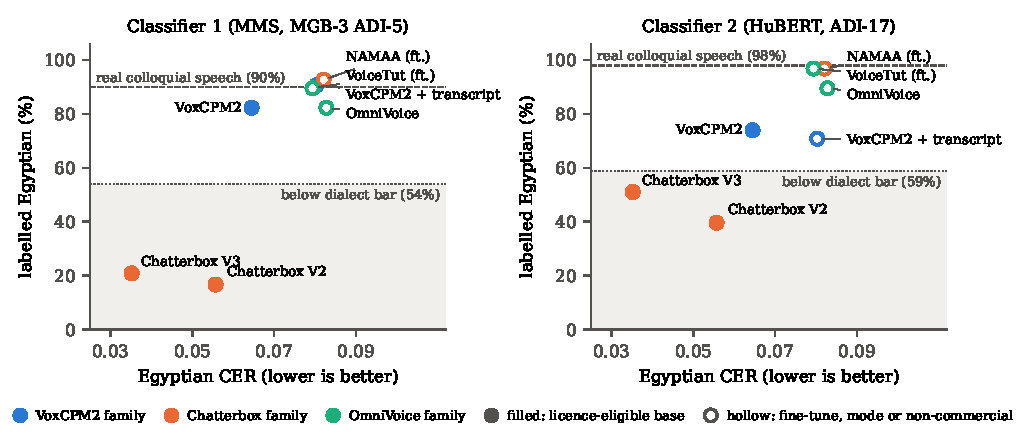
\includegraphics[width=\linewidth]{figures/dissociation.pdf}
\caption{Egyptian CER against the share labelled Egyptian under two dialect classifiers (bake-off). Shaded: below the
dialect bar. The two lowest-CER systems are the two least Egyptian.}
\label{fig:dissociation}
\end{figure}

\paragraph{Lowest CER, least Egyptian}
\cbthree has the lowest CER of all systems (\R{bk:cb-v3:cer}; \cref{tab:bakeoff,fig:dissociation}) and Chatterbox~V2 the
second lowest (\R{bk:cb-v2:cer}). Classifier~1 labels only \R{bk:cb-v3:c1pct} and \R{bk:cb-v2:c1pct} of their outputs
Egyptian, against \R{cal:lahgtna:c1pct} for real colloquial speech; most of the rest is labelled Levantine
(\R{lab:cb-v3:Levantine} for V3), Gulf (\R{lab:cb-v3:Gulf}) or MSA (\R{lab:cb-v3:MSA}). \vox has a higher CER
(\R{bk:voxcpm2:cer}), with an overlapping interval, and is labelled Egyptian \R{bk:voxcpm2:c1pct} of the time. Similarity
and predicted quality do not separate the bases either: \cbthree has the highest DNSMOS of the three eligible bases and
Chatterbox~V2 the highest similarity.

\paragraph{What each metric would choose}
Point estimates on 96 utterances could pick a winner by chance, so we ask how often a selection rule fails. In each of
\R{sel:B} bootstrap resamples of texts and voices we apply each rule and record whether its choice clears the dialect bar
(\cref{tab:selection}). Among the three eligible bases, every standard metric picks a Chatterbox model:
the choice of lowest CER fails the bar in \R{sel:eligible:cer:fail1} of resamples under classifier~1 and
\R{sel:eligible:cer:fail2} under classifier~2, highest similarity in \R{sel:eligible:ecapa:fail1} and
\R{sel:eligible:ecapa:fail2}, highest predicted quality in \R{sel:eligible:dnsmos:fail1} and
\R{sel:eligible:dnsmos:fail2}. Lowest CER among systems that clear the bar picks \vox in
\R{sel:eligible:amended:pickshare} of resamples. Across all nine configurations, lowest CER still fails the bar in
\R{sel:all:cer:fail1} of resamples, while highest similarity happens to pick a non-commercial model that clears it: the
metrics are not anti-correlated with the dialect, they carry no information about it, so what they pick depends on the
pool.

\begin{table*}[t]
\centering\small
\begin{adjustbox}{max width=\textwidth}
\rawinput{../generated/tab_selection.tex}
\end{adjustbox}
\caption{What each selection rule picks over \R{sel:B} two-way bootstrap resamples of the bake-off (texts and voices
resampled, the same draw for every system). Picked: share of resamples in which the rule chose that system. Fails bar:
share of resamples in which the rule's choice, whichever it was, falls below the dialect bar. Last row: CER ranking among
the systems that clear the bar (the amended G1). $^\dagger$Non-commercial weights.}
\label{tab:selection}
\end{table*}

\paragraph{Three seeds on held-out sentences}
On the 24 held-out sentences with three seeds each, \vox and \cbthree cannot be told apart by CER (paired difference
\R{pt:voxcpm2_minus_cb-v3:egy_main:cer_best:diff}, 95\% CI \R{pt:voxcpm2_minus_cb-v3:egy_main:cer_best:ci}) or similarity
(\R{pt:voxcpm2_minus_cb-v3:egy_main:sim_ecapa:diff}, CI \R{pt:voxcpm2_minus_cb-v3:egy_main:sim_ecapa:ci}), and DNSMOS
prefers \cbthree. The Egyptian share separates them by \R{pt:voxcpm2_minus_cb-v3:egy_main:c1:diff} under classifier~1
(CI \R{pt:voxcpm2_minus_cb-v3:egy_main:c1:ci}) and \R{pt:voxcpm2_minus_cb-v3:egy_main:c2:diff} under classifier~2 (CI
\R{pt:voxcpm2_minus_cb-v3:egy_main:c2:ci}).

\paragraph{No relation across systems}
Across the nine configurations, the rank correlation between CER and the Egyptian share is \R{sel:rhoc1} under
classifier~1 (bootstrap interval \R{sel:rhoc1:ci}) and \R{sel:rhoc2} under classifier~2 (\R{sel:rhoc2:ci}). Nine systems
cannot rule out a moderate relation in either direction; the selection analysis is the direct test.

\paragraph{Two classifiers and the reference voices}
Classifier~2, trained on different speech with a different backbone and label set, is more generous to every system but
ranks the systems in nearly the same order (Spearman $\rho=\R{rank:c1c2:rho}$), and under it too both Chatterbox bases
fall below the bar while \vox clears it. Splitting the bake-off by the dialect of the reference clip does not remove the
gap under classifier~1: with the references labelled Egyptian by both classifiers, \cbthree is labelled Egyptian
\R{ref:cb-v3:egy:c1} of the time and \vox \R{ref:voxcpm2:egy:c1}; with references labelled MSA,
\R{ref:cb-v3:msa:c1} and \R{ref:voxcpm2:msa:c1}. Classifier~2 is more sensitive to the reference: with Egyptian
references it labels \cbthree Egyptian \R{ref:cb-v3:egy:c2} of the time against \R{ref:voxcpm2:egy:c2} for \vox, a smaller
gap than with MSA references. Per utterance the two classifiers agree moderately (Cohen's $\kappa=\R{kappa:gen}$ on
generated speech), so we rely on system-level shares.

\paragraph{Which features are lost}
The classifiers say that the dialect is wrong, not what is wrong. After the main results we therefore looked at two
textbook markers of Egyptian Arabic: jiim, [g] in Egyptian and [\textipa{dZ}] or [\textipa{Z}] in MSA and the Levantine
and Gulf dialects, and qaaf, a glottal stop in Egyptian (as in urban Levantine) and [q] in MSA. A multilingual phone
recogniser \citep{xu2022phoneme} transcribes every clip; we count the share of [g] among the recognised [g],
[\textipa{dZ}] and [\textipa{Z}] in clips whose text contains jiim, and the recognised [q] per qaaf letter
(\cref{tab:features}). As the counts are not aligned to the letters, they are calibrated on real speech: real colloquial
Egyptian has jiim as [g] \R{df:lahgtna_eg:jiim} of the time and \R{df:lahgtna_eg:qaaf} [q] per qaaf, while Egyptian
speakers reading the mostly MSA FLEURS texts keep the [g] (\R{df:fleurs_ar_eg:jiim}) but say qaaf as [q]
(\R{df:fleurs_ar_eg:qaaf}). \cbthree and Chatterbox~V2 say jiim as [g] only \R{df:cb-v3:jiim} and \R{df:cb-v2:jiim} of
the time and keep [q] for qaaf (\R{df:cb-v3:qaaf} and \R{df:cb-v2:qaaf}); \vox is at the level of real colloquial speech
(\R{df:voxcpm2:jiim} and \R{df:voxcpm2:qaaf}; \vox $-$ \cbthree \R{df:d:voxcpm2-cb-v3:jiim} points for jiim, CI
\R{df:d:voxcpm2-cb-v3:jiim:ci}). Across the nine configurations the jiim measure orders the systems like the classifiers
(Spearman \R{df:rho:c1} and \R{df:rho:c2}) and not like CER (\R{df:rho:cer}). The Chatterbox outputs thus combine a
non-Egyptian jiim with an MSA qaaf, which fits the Levantine, Gulf and MSA labels they receive.

\begin{table}[t]
\centering\small
\begin{adjustbox}{max width=\linewidth}
\rawinput{../generated/tab_features.tex}
\end{adjustbox}
\caption{Two markers of Egyptian Arabic in the outputs, from a phone recogniser: share of [g] among recognised [g],
[\textipa{dZ}] and [\textipa{Z}] in clips whose text has jiim (Egyptian [g]), and recognised [q] per qaaf letter
(Egyptian [\textipa{P}], MSA [q]). Two-way bootstrap 95\% intervals (real speech: over clips). Added after the main
results.}
\label{tab:features}
\end{table}

\paragraph{Why}
The pattern fits the training data rather than the architecture: the Chatterbox systems without documented Egyptian
training data are labelled Levantine more than anything else, while NAMAA, a Chatterbox fine-tune on Egyptian speech, is
labelled Egyptian \R{bk:namaa:c1pct} of the time. A recogniser trained mostly on MSA and pan-Arabic data transcribes
Levantine- or MSA-accented Egyptian sentences correctly: the words survive, the dialect does not, and CER cannot see the
difference.

\section{Native listeners agree}\label{sec:listeners}

\begin{table}[t]
\centering\small
\begin{adjustbox}{max width=\linewidth}
\rawinput{../generated/tab_listening.tex}
\end{adjustbox}
\caption{Blind listening test (\R{mlt:n} native Egyptian listeners after quality control). Mean rating with
listener-and-sentence bootstrap 95\% interval; ``wrong word heard'': share of clips with a reported wrong, missing or
garbled word; ``same speaker'': similarity to a second real clip of the cloned speaker (one pair per system and listener).}
\label{tab:listening}
\end{table}

\R{mlt:complete} native Egyptian listeners who were not involved in the work each rated 24 generated sentences (six per
system, Latin square over sentences and voices), four real colloquial clips as a hidden anchor, two repeated clips and
four speaker-similarity pairs; \R{mlt:excl} failed both pre-specified quality checks, which leaves \R{mlt:n}
(\cref{app:listening}). Listeners heard \cbthree as much less Egyptian than \vox: \R{mlt:cb-v3:egy} against
\R{mlt:voxcpm2:egy} on a five-point scale (\cref{tab:listening}), and as less natural (\R{mlt:cb-v3:nat} against
\R{mlt:voxcpm2:nat}). In a cumulative-link mixed model with random effects for listener, voice and sentence, the
difference is \R{mlt:c:voxcpm2-cb-v3:egy:est} on the log-odds scale for Egyptian-ness (CI \R{mlt:c:voxcpm2-cb-v3:egy:ci},
\R{mlt:c:voxcpm2-cb-v3:egy:p} after Holm correction over six planned contrasts) and \R{mlt:c:voxcpm2-cb-v3:nat:est} for
naturalness. Listeners also reported a wrong, missing or garbled word in \R{mlt:cb-v3:ww} of \cbthree's clips, the most of
any system, although its CER is among the lowest: words that a recogniser trained mostly on MSA accepts can still sound
wrong to an Egyptian listener. The mean Egyptian rating orders the four systems exactly as both classifiers do (Spearman
\R{mlt:rho:c1} and \R{mlt:rho:c2}) and not as CER does (\R{mlt:rho:cer}).

\paragraph{Clip by clip}
Four systems are few for a rank correlation, so after the test we also asked, in an analysis the protocol did not plan,
whether the measures of each clip follow its ratings. Across the \R{mlc:clips} rated generated clips (\R{mlc:perclip}
ratings per clip on average), the probability of Egyptian under either classifier correlates with the mean Egyptian
rating (Spearman \R{mlc:rho:egy:p1}, CI \R{mlc:rho:egy:p1:ci}, and \R{mlc:rho:egy:p2}, CI \R{mlc:rho:egy:p2:ci};
listener-and-sentence bootstrap), and CER does not (\R{mlc:rho:egy:cer}, CI \R{mlc:rho:egy:cer:ci}). Clips that
classifier~1 labels Egyptian are rated \R{mlc:mean:egy:egy1:yes} on average, the others \R{mlc:mean:egy:egy1:no}. Within a
system the classifiers follow the listeners only weakly (\R{mlc:rhow:egy:p1} and \R{mlc:rhow:egy:p2}, with intervals that
include zero): they measure the dialect of a system, not of a single utterance, which is how we use them.

\paragraph{Robustness}
The result holds for the listeners who used
headphones or earbuds (\cbthree \R{mlt:dev:headphones_or_earbuds:cb-v3:egy}, \vox
\R{mlt:dev:headphones_or_earbuds:voxcpm2:egy}) and for those who used loudspeakers (\R{mlt:dev:loudspeaker:cb-v3:egy}
and \R{mlt:dev:loudspeaker:voxcpm2:egy}). Real speech is rated \R{mlt:real:egy}, no higher than the Egyptian systems; the real clips are spontaneous
recordings of varying quality. Agreement between listeners is moderate (Krippendorff's ordinal $\alpha$
\R{mlt:alpha:egy} for Egyptian-ness and \R{mlt:alpha:nat} for naturalness).

\section{An engine that keeps the dialect}\label{sec:engine}

\begin{table*}[t]
\centering\small
\begin{adjustbox}{max width=\textwidth}
\rawinput{../generated/tab_seeds.tex}
\end{adjustbox}
\caption{Held-out Egyptian sentences over \R{s3:nseeds} seeds per utterance (mean and two-way bootstrap 95\% interval).
NAMAA is the best Egyptian fine-tune with permissive weights; \cbthree is the lowest-CER system of the bake-off.}
\label{tab:seeds}
\end{table*}

Under a rule that applies the dialect bar before ranking on CER, \vox is the only eligible base that passes. No
Egyptian training data with an acceptable licence and provenance exists beyond two synthetic voices, so \BA keeps the
\vox weights unchanged and adds an engine around them; every default was chosen on the tuning sentences.
\emph{Number and symbol normaliser}: digits were the largest error source for every system, and the normaliser writes
cardinals, dates, times (\emph{7:30} $\rightarrow$ \ar{sab3a-wnoss}), prices, percentages and counted plurals as Cairenes
say them (\ar{khamastashar} ``fifteen'', \ar{tultumiyya} ``three hundred''), never in MSA (\ar{khamsata3ashar},
\ar{thalathumi2a}). \emph{Loanword policy}: common English loanwords in an Arabic sentence are written in Arabic script as
Egyptians say them (\emph{meeting} $\rightarrow$ \ar{meeting}), which on the tuning set kept CER level and raised the
Egyptian share from \R{cs:keep:c1pct} to \R{cs:arabic:c1pct}. \emph{Reference transcript}: \vox can condition on the
reference audio and its transcript, which in the bake-off raised similarity from \R{bk:voxcpm2:ecapa} to
\R{bk:voxcpm2-prompt:ecapa}; users rarely type what they said, so the engine transcribes the reference with Whisper
large-v3-turbo. \emph{Reference preparation}: uploads are screened for length, noise and clipping and cut to the cleanest
6--15\,s window. \emph{Long text}: sentences are packed into chunks of at most \R{chunk:maxchars} characters, and each
chunk is checked against the speaking-rate and level bands of real speech and regenerated if it fails.

On held-out sentences over three seeds (\cref{tab:seeds}), \BA lowers Egyptian CER from \R{s3:voxcpm2:egy_main:cer_best}
to \R{s3:ba:egy_main:cer_best} (paired CI \R{pt:ba_minus_voxcpm2:egy_main:cer_best:ci}) and raises similarity from
\R{s3:voxcpm2:egy_main:sim_ecapa} to \R{s3:ba:egy_main:sim_ecapa}, matching \cbthree's CER
(\R{pt:ba_minus_cb-v3:egy_main:cer_best:diff}, CI \R{pt:ba_minus_cb-v3:egy_main:cer_best:ci}) while being labelled Egyptian
far more often. Removing one component at a time (\cref{tab:ablation}) traces almost all of the measurable gain to the
automatic reference transcript (about \R{ab:share:notrans:ecapa} of the similarity gain and \R{ab:share:notrans:cer} of the
CER gain); the Egyptian number normaliser leaves CER unchanged, because a recogniser writes an Egyptian and an MSA
reading of a number as the same digits, a second instance of the same blind spot. Listeners rated \BA as Egyptian as its
base (\R{mlt:ba:egy} and \R{mlt:voxcpm2:egy}; \R{mlt:c:ba-voxcpm2:egy:est}, CI \R{mlt:c:ba-voxcpm2:egy:ci},
\R{mlt:c:ba-voxcpm2:egy:p}) and somewhat less natural (\R{mlt:ba:nat} against \R{mlt:voxcpm2:nat};
\R{mlt:c:ba-voxcpm2:nat:p}); neither difference is significant, and the intervals do not exclude a small loss of
naturalness. They reported a wrong word less often for \BA than for any other system (\R{mlt:ba:ww}), and the engine
keeps the Egyptian jiim of its base (\R{df:ba-ho:jiim} against \R{df:voxcpm2-ho:jiim}; \cref{tab:features}).

\begin{table}[t]
\centering\small
\begin{adjustbox}{max width=\linewidth}
\rawinput{../generated/tab_ablation.tex}
\end{adjustbox}
\caption{Ablations on held-out sentences (one seed, the same utterances in every row). Each middle row removes one
component; the last row is \vox used directly. Bold: the paired 95\% interval of the difference from the full engine
excludes zero. CER$_\text{canon.}$: CER after mapping spellings of the same loanword to one form.}
\label{tab:ablation}
\end{table}

\paragraph{Long text and other languages}
On 24 long passages written after the engine was frozen (8 per language, two voices each), neither system failed, and
similarity is higher with the engine in all three languages (Egyptian \R{lfp:arz:sim_ecapa:diff}, CI
\R{lfp:arz:sim_ecapa:ci}). Error rates do not separate the systems, and they expose the same blind spot inside the
recogniser: on one passage Whisper rewrites the colloquial opening into MSA and then loops, for both systems
(CER \R{lfw:clip:ba:arz05:win} and \R{lfw:clip:voxcpm2:arz05:win}), so we draw no conclusion about long-form Egyptian CER.
In English and French the engine passes every bar of the protocol (WER \R{ho:ba:en:wer} and \R{ho:ba:fr:wer}).

\section{Recommendations}\label{sec:recommendations}
For the evaluation of speech generation in a dialect, our results suggest five practices, each cheap next to training a
model. (i) \emph{Calibrate every metric on real dialectal speech}, including CER and predicted quality, so that a score
can be read against what real speakers obtain (\cref{tab:calibration}). (ii) \emph{Fix a dialect bar relative to real
speech before the first model is run}, and apply it before ranking on any other metric; a rule that ranks first and
checks the dialect afterwards picks the wrong model (\cref{tab:selection}). (iii) \emph{Use at least two dialect
classifiers trained on different data}, and read them at the level of systems, where they agree with each other and
with listeners, not of single utterances. (iv) \emph{Check named markers of the dialect}, such as the Egyptian jiim,
with a phone recogniser calibrated on real speech: they show what is wrong and give developers something to fix
(\cref{tab:features}). (v) \emph{Let native listeners check the decision} in a blind test with real-speech anchors,
repeats and quality criteria fixed in advance; \R{mlt:n} listeners were enough to confirm a large difference
(\cref{tab:listening}).

\section{Conclusion}
For Egyptian Arabic voice cloning, intelligibility, speaker similarity and predicted quality do not see the dialect. Used
to choose a base among licence-eligible open models, each of them picks a model that fails a dialect bar calibrated on
real colloquial speech, and native listeners hear that model as far less Egyptian, exactly as two independent
classifiers do. For any dialect, evaluations of speech generation should report a dialect measure calibrated on real
dialectal speech next to error rates, fix the dialect bar before the first model is run, and let native listeners check
the decision.

\section*{Limitations}
The listening test has \R{mlt:n} listeners after quality control, enough for the large difference between \vox and
\cbthree but not to show that the engine and its base are equivalent; agreement is moderate, and most listeners come from
Upper Egypt. It deviates from its protocol in three ways (\cref{app:listening}): the cloned voices are the FLEURS speakers
of the held-out set rather than consenting volunteers, loudspeakers were accepted besides headphones (results do not
change with the device), and three of twelve counterbalanced lists have no complete session. The reference voices are
read FLEURS speech in an MSA register, and six voices make every interval wide; colloquial references would show how much
a colloquial reference helps each model. Two classifiers were used, both trained on broadcast or web speech; the second
was added after the first results, and the clip-level analysis after the listening test. The work covers one dialect, short sentences and long passages in three languages,
and models available in November 2026.

\section*{Ethical considerations}
\paragraph{Listening test}
Native Egyptian adults took part as unpaid volunteers. The first page of the test stated the purpose of the study, that taking
part was voluntary and could be stopped at any time by closing the page, what would be stored, and that results would be
published only in aggregate, and it gave a contact address; listeners confirmed that they were 18 or older and agreed to
take part before the first clip. The test asked for no name or contact details and stored no IP address, only a random
session identifier, the ratings and four coarse descriptors (age band, gender, governorate, listening device);
individual answers are not published. Listeners heard speech cloned from FLEURS speakers and real clips from a public
corpus, and no new recordings of people were made. No institutional ethics review was sought: taking part was anonymous, voluntary and unpaid, consisted only of listening to short clips and rating them, carried no foreseeable risk beyond those of everyday life, and collected no information that identifies a person.

\paragraph{Voice cloning}
Voice cloning can impersonate people. The engine's public demo requires a consent statement, does not store uploads, and
watermarks every output with AudioSeal \citep{sanroman2024audioseal}; FLEURS reference clips and the audio cloned from
them are used for measurement only and are not redistributed.

\paragraph{Use of AI assistants}
An AI assistant (Claude) helped write the code of the experiments and analyses and draft and edit parts of the text. The
authors reviewed all of it and take full responsibility for the content; every number is produced by scripts from the
results files.

\bibliography{../refs}

\appendix
\section{Metrics on real speech}\label{app:calibration}
\begin{table}[h]
\centering\small
\begin{adjustbox}{max width=\linewidth}
\rawinput{../generated/tab_calibration.tex}
\end{adjustbox}
\caption{Metrics on calibration speech. lahgtna-v2: real colloquial Egyptian; FLEURS: read Egyptian, mostly MSA in
register; NileTTS: synthetic colloquial speech, for comparison only.}
\label{tab:calibration}
\end{table}

\section{Listening test: design and deviations}\label{app:listening}
Each of 12 counterbalanced lists has two practice clips (not analysed), 24 generated clips on 24 different held-out
sentences (six per system; sentence $k$ of list $l$ is spoken by system $(k+l) \bmod 4$, the voice rotating with $l$),
four real colloquial clips, two repeats of generated clips and four speaker-similarity pairs. Clips are trimmed of
silence and normalised to $-23$\,LUFS; names are hidden and the order is random. Listeners rate how Egyptian a clip sounds
(1, not Egyptian at all, to 5, a native Egyptian speaker) and how natural it is (1, clearly machine, to 5, completely
natural), and say whether a word was wrong, missing or garbled. Listeners were adults who grew up in Egypt and speak
Egyptian Arabic natively, recruited through personal networks and unpaid. Unfinished sessions (\R{mlt:unfinished}) and one test
session by an author are excluded. The quality checks, made concrete before any system score was computed: the
real-speech check passes when at least two of the four real clips are rated 4 or more on both scales, the consistency
check when at least one repeat is within one point of its first rating on both scales; a listener failing both is
excluded. Analysis as pre-specified: cumulative-link mixed models (R package \texttt{ordinal}) with random intercepts for
listener, voice and sentence, Holm correction over six contrasts, two-way bootstrap intervals and Krippendorff's ordinal
$\alpha$. Each listener contributes the 24 generated clips of the list; practice clips and repeats (used only for the
consistency check) are not analysed. The clip-level analysis of \cref{sec:listeners} was added after the test: the mean
rating of each clip against its CER and classifier probabilities, with intervals from the same two-way bootstrap, and for
the within-system values every measure and rating centred on its system mean. Deviations from the protocol: the voices are the six FLEURS speakers of the held-out set rather than volunteers'
recordings; 36 ratings per listener instead of the sketched 60; loudspeakers accepted; collection stopped at 20 complete
sessions, with lists assigned in turn to every session started.

\end{document}
